\documentclass{article} % For LaTeX2e
\usepackage{nips13submit_e,times}
\usepackage{hyperref}
\usepackage{url}
\usepackage{verbatim}
\usepackage{graphicx}
\usepackage{subcaption}
\usepackage{listings}
\usepackage{clrscode4e}
\usepackage{tikz}
\usepackage{amsmath}


%\documentstyle[nips13submit_09,times,art10]{article} % For LaTeX 2.09


\title{Incremental Construction of Programs in a Multitask Setting}

\begin{comment}
\author{
David S.~Hippocampus\thanks{ Use footnote for providing further information
about author (webpage, alternative address)---\emph{not} for acknowledging
funding agencies.} \\
Department of Computer Science\\
Cranberry-Lemon University\\
Pittsburgh, PA 15213 \\
\texttt{hippo@cs.cranberry-lemon.edu} \\
\And
Coauthor \\
Affiliation \\
Address \\
\texttt{email} \\
\AND
Coauthor \\
Affiliation \\
Address \\
\texttt{email} \\
\And
Coauthor \\
Affiliation \\
Address \\
\texttt{email} \\
\And
Coauthor \\
Affiliation \\
Address \\
\texttt{email} \\
(if needed)\\
}
\end{comment}
% The \author macro works with any number of authors. There are two commands
% used to separate the names and addresses of multiple authors: \And and \AND.
%
% Using \And between authors leaves it to \LaTeX{} to determine where to break
% the lines. Using \AND forces a linebreak at that point. So, if \LaTeX{}
% puts 3 of 4 authors names on the first line, and the last on the second
% line, try using \AND instead of \And before the third author name.

\newcommand{\fix}{\marginpar{FIX}}
\newcommand{\new}{\marginpar{NEW}}

%\nipsfinalcopy % Uncomment for camera-ready version

\begin{document}


\maketitle

\begin{abstract}
How can machine learning techniques be used to solve problems whose solutions are best represented as computer programs? For example, suppose a researcher wants to design a probabilistic graphical model for a novel domain. Searching the space of probabilistic models automatically is notoriously difficult and is especially difficult when the latent variables are possible. However, when researchers seem able to relatively easily adapt commonly used modeling motifs to new domains. In doing so, they draw on abstractions such as trees, chains, grids and plates to constrain and direct the kinds of models they produce. This suggests that before we ask machine learning algorithms to discover parsimonious models of new domains, we should develop techniques that enable our algorithms to automatically learn these ``graphical conepts'' in much the same way that researchers themselves do, by seeing examples in the literature. One natural way to think of these graphical concepts is as programs that take sets of random variables and produce graphical models that relate them. In this work, we describe the SEC algorithm, which attempts to learn a distribution over programs by incrementally finding program components that commonly help to solve problems in a given domain, and we show prelimarily that SEC is able to discover the graphical concepts that underlie many of the common graphical model structures.  
\end{abstract}


\section{Introduction}


The vast majority of research in machine learning is focused on utilizing large amounts of noisy data living in high-dimensional, real-valued vector spaces. Such research has been immensely successful and has enabled automatic and accurate modelling on a scale that was previously infeasible. However, when we want to build a car, draw a painting, or design the machine learning models to which we apply our new algorithms and techniques, we face problems that current machine learning tools are unable to handle. The highly structured objects that humans produce seems to require a different representation than the ones which machine learning algorithms have most successfully employed. 

To address this problem, many structured representations have been proposed in the machine learning and AI literatures: learning over graphs \cite{}, grammars\cite{}, Horn clauses\cite{}, relations{}, etc., has been investigated. These are representations that attempt to bridge the gap between the tractablity of learning and reasoning in smooth continuous spaces and the expressivity of general purpose programming languages. 

However, many of the most natural representations of structured domains are best described as programs and are difficult to fit into more restrictive representations.  To take an example directly from the machine learning literature, consider the plate notation~\cite{DBLP:journals/jair/Buntine94} commonly used to describe graphical models over collections of variables. A typical example is shown in Figure~\ref{fig:lda_plate}~\cite{DBLP:journals/jmlr/BleiNJ03}. The goal of plate notation is precisely to express the notion of a ``for loop'' within the graphical model representation. One reason this is a convenient tool is that researchers conceptualize their models as sampling procedures -- easily expressed as programs (see Figure~\ref{fig:lda_code}, but not as static graphs -- and can use plate notation to express a commonly occuring control structure. In fact, the field of probabilistic programming, which has gained recent popularity, is spurred on by exactly the motivation that our models are most naturally expressed as programs. 

Suppose, then, that we want to create machine learning algorithms that can help discover good models for data in novel domains; that is, we want algorithms that discovers the structure of the latent graphical model underlying the data. This is a field of active research \ 

In this paper, we describe our approach to learning over structured representations as a search over the space of programs in a functional programming language. We characterize learning in this space as incrementally developing a weighted library of program abstractions, i.e. a collection of subroutines, that are commonly used to solve problems in a given domain. The SEC algorithm (for Sequential Exploration-Compression), which we present here, takes a set of related tasks and produces a distribution over programs that solve those tasks; as it refines this distribution, SEC is able to search the space of programs more efficiently and solve more tasks. 

We will present here two domains of interest. First, continuing with the example above, we will describe how SEC can learn to efficiently explore the space of relevant graphical models for a given problem. Second, we will examine SEC's performance on a completely different type of task, in which we want to an algorithm to build tall and physically stable block towers. 

\lstset{
	basicstyle=\scriptsize\ttfamily,
    commentstyle=\color{white!40!black},
    escapechar=+,
    escapebegin=\color{white!40!black},
    escapeend={},
    keywordstyle=\bfseries\color{Periwinkle},
    numbers=left,
    numberstyle=\sffamily\tiny\color{gray},
}


\begin{figure}[h]
\centering
\begin{subfigure}{.5\textwidth}
  \centering
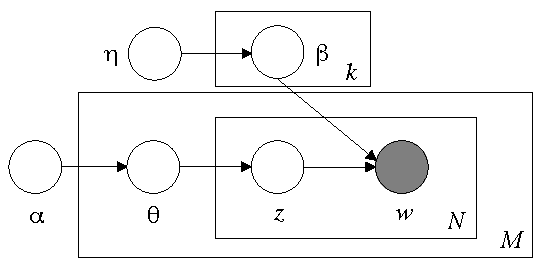
\includegraphics[width=.7\linewidth]{./figures/lda_plate_blei.pdf}
  \caption{An example of typical plate notation use. \label{fig:lda_plate}}

\end{subfigure}%
\begin{subfigure}{.4\textwidth}
	\begin{lstlisting}[frame=single, numbers=none, xleftmargin=0pt]
	for +$k$+ = 1:NumTopics
	  +$\beta$+[k] +$\sim$+ Dirichlet(+$\eta$+)
	for m = 1:NumDocuments
	  +$\theta$+[m] +$\sim$+ Dirichlet(+$\alpha$+) 
	  for n = 1:NumWords 
	    z +$\sim$+ Categorical(+$\theta$+[m])
	    w+$\sim$+ Categorical(+$\beta$+[z])
	\end{lstlisting}
  \caption{The same model as a program.}
  \label{fig:lda_code}
\end{subfigure}
\caption{The popular Latent Dirichlet Allocation model in two forms.}
\label{fig:lda}
\end{figure}


\section{The SEC Algorithm}
\subsection{Generative Model}
We propose a generative model over programs that captures two intuitions:
\begin{itemize}
\item{Useful programs are composed of useful subparts.}
\item{Short programs are a prior more likely.}
\end{itemize}
\begin{codebox}
\li \id{G} $\sim$ $P_G(\cdot)$ \Comment{Draw grammar from description-length prior}
\li \id{\ell_n} $\sim\mbox{Uniform}(1, L)$ \Comment{Draw number of subprograms in $n^{th}$ program}
\li \Comment{Draw $\rho_n$, the $n^{th}$ program, by composing its subprograms, $e_n^{i}$}
\li \id{e_n^{i}} $\sim P_{e|G}(\cdot | G)$
\li \id{\rho_n} $= e_n^{\ell_n} (e_n^{\ell_n-1} ( \cdots e_n^{1}))$
\li \Comment{Draw $t_n$ by adding noise $\epsilon_n$ to the output of $\rho_n$}
\li \id{\epsilon_n} $\sim P_{\mbox{noise}}(\cdot)$
\li \id{t_n} $= \rho_n + \epsilon_n$
\end{codebox}


Write down the generative model. Connect to EC and Percy Liang's work. Discuss ``programs as plans.''
\subsection{Inference}
We implement an iterative Expectation-Maximization algorithm that performs MAP estimation of the libraray, $G$, given the tasks, $\{t_n\}$.
The joint distribution factorizes as
\begin{equation}
P(G,\{\rho_n\},\{t_n\}) = \frac{1}{L^N} P(G) \prod_n P(t_n | \rho_n) \prod_i P(e^i_n | G)
\label{eq:joint}
\end{equation}
From equation (\ref{eq:joint}), the EM updates are
\begin{eqnarray}
q(\rho_n) &\propto& P(t_n | \rho_n) \prod_i P(e^i_n | G^{old})\\
\label{eq:qdist}
G^{new} &=& \operatorname{argmin}_G \left( -\ln P(G) -
\sum_n 
E_{q_n}
 \left[ \ln P(\rho_n | G) \right] \right)
 \label{eq:gmax}
\end{eqnarray}
Exact computation of $q(\cdot)$ in equation (\ref{eq:qdist}) would involve marginalizing over the space of all programs.
Instead, we perform a heuristic search over the space of programs, with the goal of finding those programs for which $q(\cdot)$ is high.
Rather than use mutation and crossover operators, as done in genetic programming, or random resampling of subprograms, as done in recent work in applying Metropolis-Hastings to program learning, we propose that the search moves should themselves be programs drawn from the grammar $G$.
Concretely, in order to modify a program $e$ to produce new candidate programs, we draw a new function from our grammar, $G$, and apply that new function to $e$.
Thus, we use the grammar not only as a distribution over programs of interest, but also as a distribution over programs that take as input other programs.
This incremental construction of programs by repeatedly applying draws from the grammar mirrors the construction of programs in the generative model.

In our experiments, we used beam search. The objective function was the unnormalized posterior $P_{t_n|\rho_n}(t_n | \cdot )P_{\rho_n | G}(\cdot | G)$.
The beam was initialized to be the programs with the highest prior probability according to the grammar $G$.
Similarly, the search moves considered were those functions with the most highest prior probability under $G$.

Equation (\ref{eq:gmax}) has a natural interpretation as a form of compression.
Interpreting negative log probabilities as description lengths, the update (\ref{eq:gmax}) picks the grammar minimizing the sum of the description length of the grammar, plus the expected description length of the programs found to solve the tasks.

Performing the minimization operation in equation (\ref{eq:gmax}) is generally difficult.
We approximate the description length of the grammar by the number of unique program fragments in the grammar, multiplied by a regularization constant.
The description length of a program is approximated by the number of (not necessarily unique) program fragments in its smallest parse tree given the grammar.
A slight generalization of the Neville-Manning algorithm then permits tractible minimization of (\ref{eq:gmax}).
Estimation of the production probabilities of $G$ is performed as in \cite{ijcai}.

\subsection{Program Representation}

Following~\cite{DBLP:conf/ijcai/DechterMAT13} and~\cite{DBLP:conf/icml/LiangJK10}, we use a
simply typed combinatory calculus -- a variable-free subset of the
polymorphic simply-typed lambda calculus~\cite{DBLP:books/daglib/0005958} -- as our
program representation language. The simplicity the combinatory calculus makes describing a distribution over its expressions particularly simple. A more detailed explanation and discussion of this program representation can be found in the papers cited above. 

\section{Application to Structure Learning}
Learning the structure of graphical models is a difficult problem - not only for machines, but also for humans, where expert knowledge is often required.
In practice, the sorts of graphical models that humans design, such as Hidden Markov Models, phylogenetic trees, topic models, and Ising models, exhibit certain symmetries and recursive structures that are amenable to synthesis by programs.
Could an algorithm, such as SEC, automatically learn these structures?

\section{Application to Graphical Model Structure Learning}

Learning the structure of graphical models that capture the independencies underlying a dataset is an active area of research\cite{adams-wallach-ghahramani-2010a}\cite{ISI:000240797500002}\cite{ISI:000178037200004}\cite{ISI:A1995RX35400001}. Graphical model structures enforce the conditional independences a modeler believes exists among latent and observed random variables\cite{DBLP:books/daglib/0066829}. 

\subsection{Graph Combinators}

Diagrams illustrating the graph combinators. An example program that makes an Ising model.

\subsection{Learning Graphical Models}

Show the actual results for our test cases: ``density estimation of the space of interesting graphical models.''
In future work, could be used as high-level moves in the search for a good structure.
Connect to, eg, Charles Kemp's work.

\begin{figure}
\begin{minipage}[c][8cm][t]{.4\textwidth}
  \vspace*{\fill}
  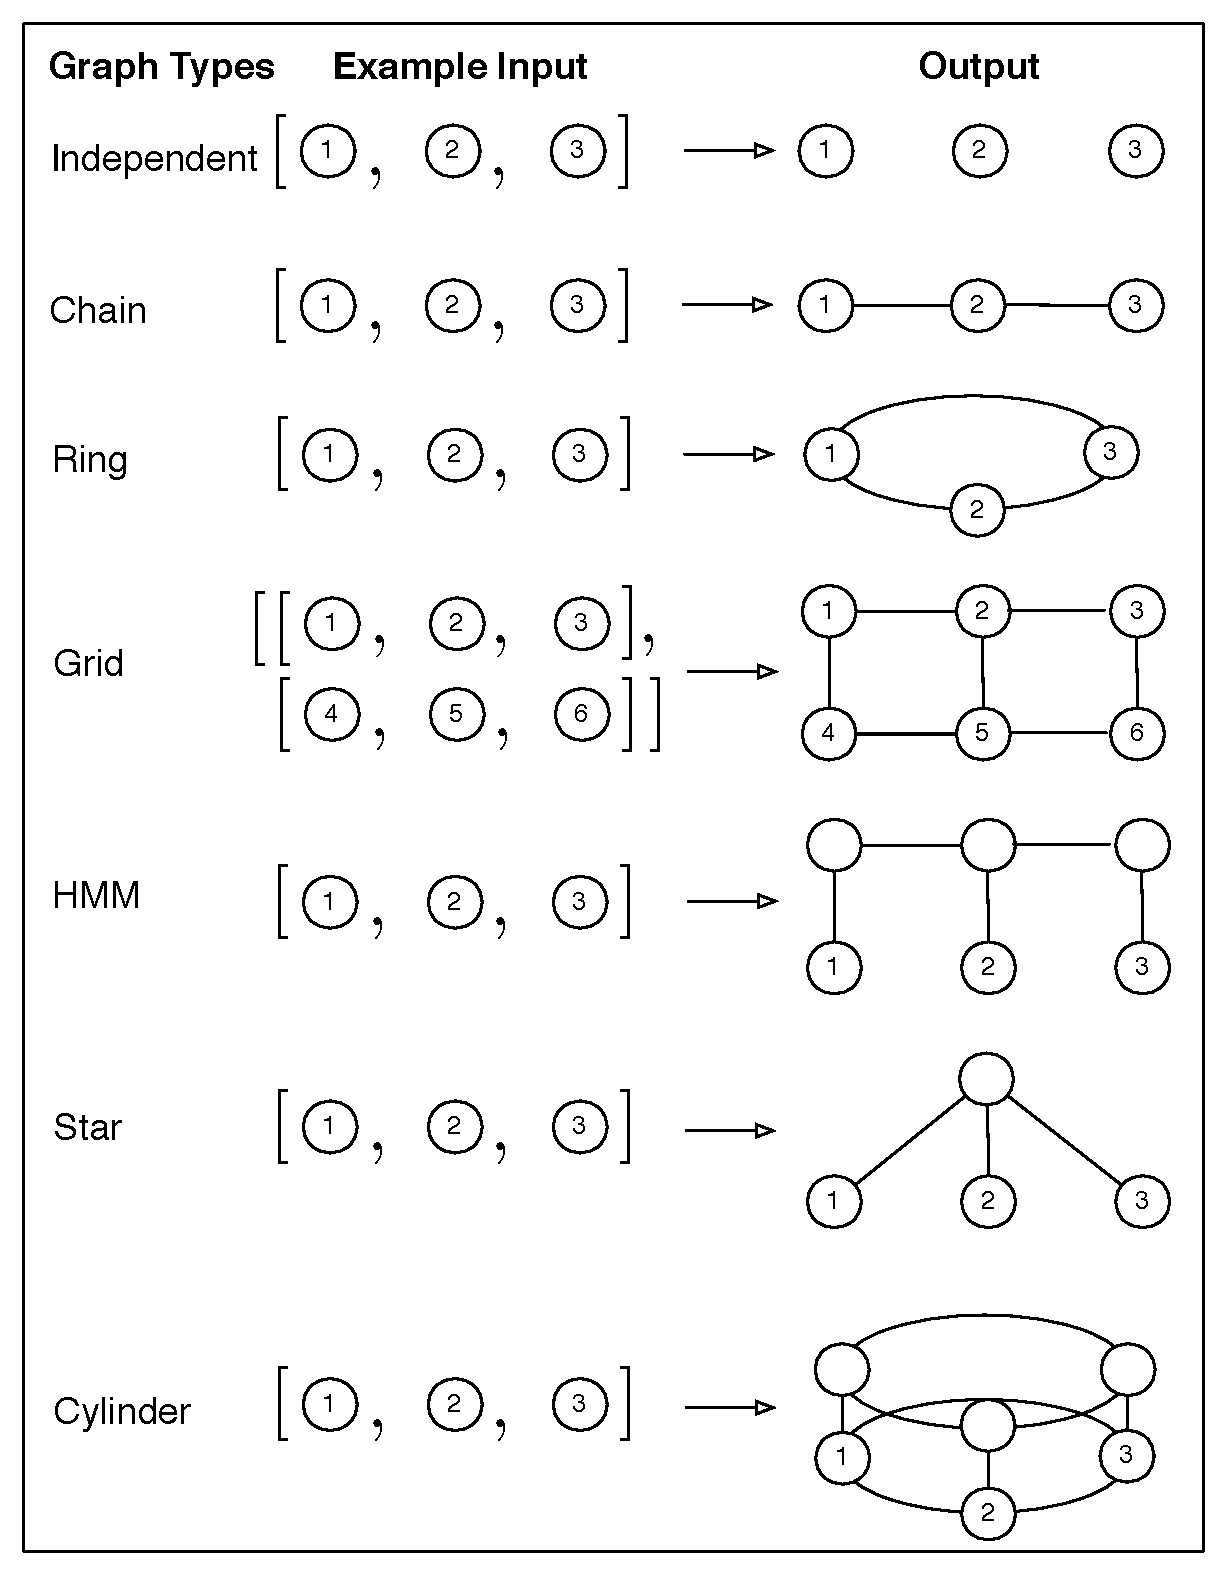
\includegraphics[width=\linewidth]{./figures/tasks.pdf}
  \caption{test figure one}
  \label{fig:test1}
\end{minipage}%
\begin{minipage}[c][8cm][t]{.3\textwidth}
  \vspace*{\fill}
  \fbox{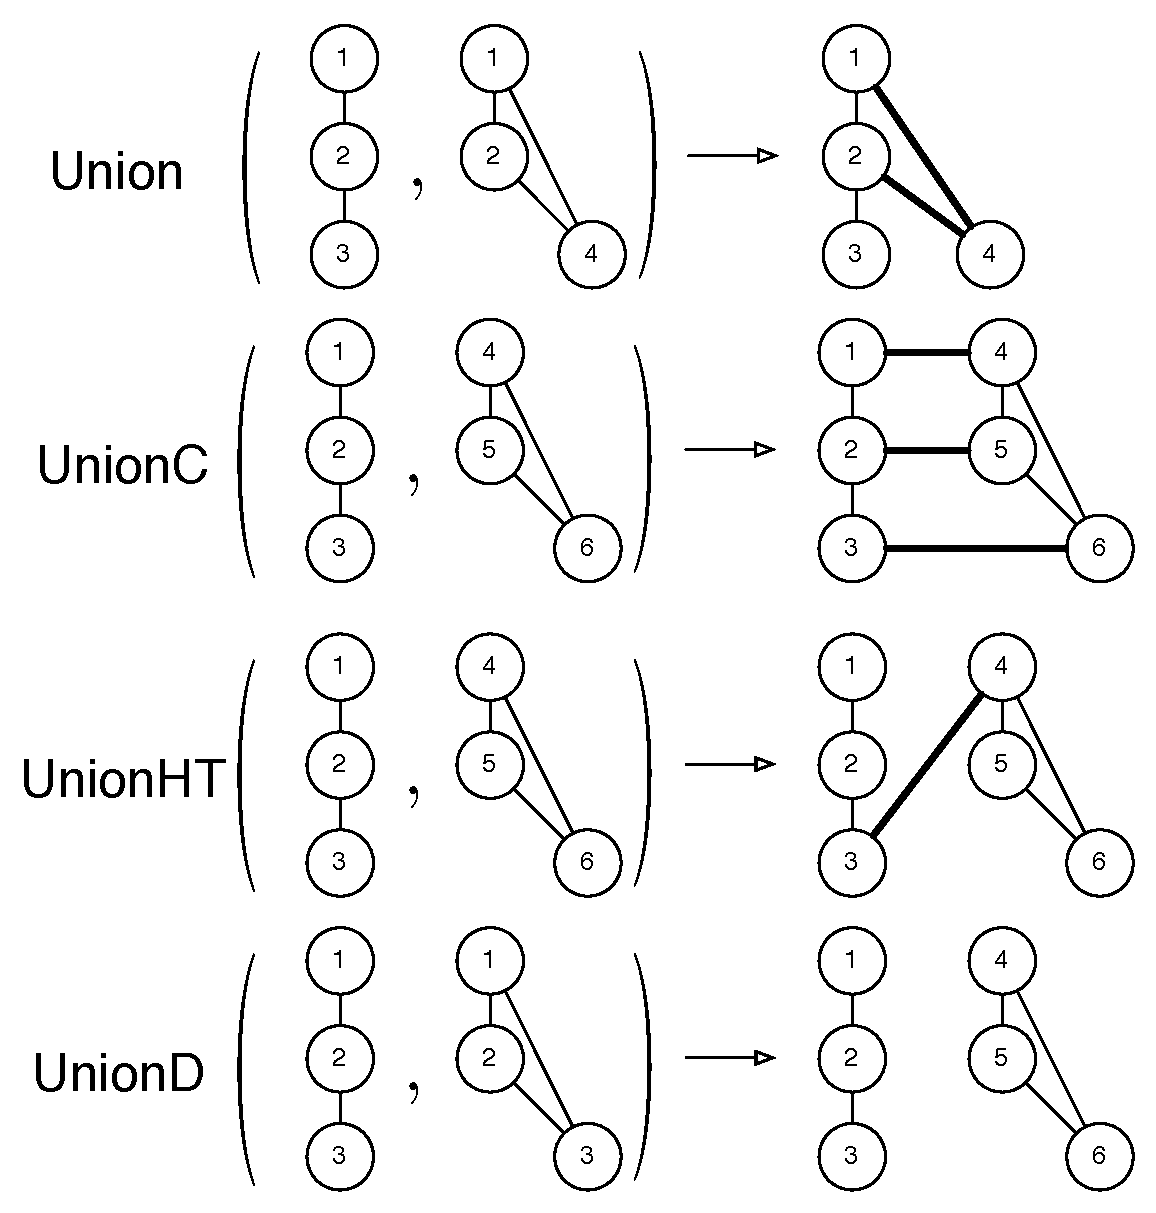
\includegraphics[width=\linewidth]{./figures/GraphCombinators.pdf}}
  \caption{test figure two}
  \label{fig:test2}\par\vfill
  % \includegraphics[width=5cm,height=4.5cm]{im
  \caption{test figure three}
  \label{fig:test3}
\end{minipage}
\end{figure}

\section{Discussion}

\subsection{Relation to Prior Work}

MH sampling of programs, ILP, Kitzelman, graph grammars

\subsection{Limitations of SEC}

Does not look at data. Does everything top-down. Blind to the utility of trying one program versus another (no active learning)


\bibliographystyle{plain}
\bibliography{eyal_bib}

\end{document}
